% Options for packages loaded elsewhere
\PassOptionsToPackage{unicode}{hyperref}
\PassOptionsToPackage{hyphens}{url}
%
\documentclass[
]{article}
\usepackage{lmodern}
\usepackage{amssymb,amsmath}
\usepackage{ifxetex,ifluatex}
\ifnum 0\ifxetex 1\fi\ifluatex 1\fi=0 % if pdftex
  \usepackage[T1]{fontenc}
  \usepackage[utf8]{inputenc}
  \usepackage{textcomp} % provide euro and other symbols
\else % if luatex or xetex
  \usepackage{unicode-math}
  \defaultfontfeatures{Scale=MatchLowercase}
  \defaultfontfeatures[\rmfamily]{Ligatures=TeX,Scale=1}
\fi
% Use upquote if available, for straight quotes in verbatim environments
\IfFileExists{upquote.sty}{\usepackage{upquote}}{}
\IfFileExists{microtype.sty}{% use microtype if available
  \usepackage[]{microtype}
  \UseMicrotypeSet[protrusion]{basicmath} % disable protrusion for tt fonts
}{}
\makeatletter
\@ifundefined{KOMAClassName}{% if non-KOMA class
  \IfFileExists{parskip.sty}{%
    \usepackage{parskip}
  }{% else
    \setlength{\parindent}{0pt}
    \setlength{\parskip}{6pt plus 2pt minus 1pt}}
}{% if KOMA class
  \KOMAoptions{parskip=half}}
\makeatother
\usepackage{xcolor}
\IfFileExists{xurl.sty}{\usepackage{xurl}}{} % add URL line breaks if available
\IfFileExists{bookmark.sty}{\usepackage{bookmark}}{\usepackage{hyperref}}
\hypersetup{
  pdftitle={asda},
  hidelinks,
  pdfcreator={LaTeX via pandoc}}
\urlstyle{same} % disable monospaced font for URLs
\usepackage[margin=1in]{geometry}
\usepackage{color}
\usepackage{fancyvrb}
\newcommand{\VerbBar}{|}
\newcommand{\VERB}{\Verb[commandchars=\\\{\}]}
\DefineVerbatimEnvironment{Highlighting}{Verbatim}{commandchars=\\\{\}}
% Add ',fontsize=\small' for more characters per line
\usepackage{framed}
\definecolor{shadecolor}{RGB}{248,248,248}
\newenvironment{Shaded}{\begin{snugshade}}{\end{snugshade}}
\newcommand{\AlertTok}[1]{\textcolor[rgb]{0.94,0.16,0.16}{#1}}
\newcommand{\AnnotationTok}[1]{\textcolor[rgb]{0.56,0.35,0.01}{\textbf{\textit{#1}}}}
\newcommand{\AttributeTok}[1]{\textcolor[rgb]{0.77,0.63,0.00}{#1}}
\newcommand{\BaseNTok}[1]{\textcolor[rgb]{0.00,0.00,0.81}{#1}}
\newcommand{\BuiltInTok}[1]{#1}
\newcommand{\CharTok}[1]{\textcolor[rgb]{0.31,0.60,0.02}{#1}}
\newcommand{\CommentTok}[1]{\textcolor[rgb]{0.56,0.35,0.01}{\textit{#1}}}
\newcommand{\CommentVarTok}[1]{\textcolor[rgb]{0.56,0.35,0.01}{\textbf{\textit{#1}}}}
\newcommand{\ConstantTok}[1]{\textcolor[rgb]{0.00,0.00,0.00}{#1}}
\newcommand{\ControlFlowTok}[1]{\textcolor[rgb]{0.13,0.29,0.53}{\textbf{#1}}}
\newcommand{\DataTypeTok}[1]{\textcolor[rgb]{0.13,0.29,0.53}{#1}}
\newcommand{\DecValTok}[1]{\textcolor[rgb]{0.00,0.00,0.81}{#1}}
\newcommand{\DocumentationTok}[1]{\textcolor[rgb]{0.56,0.35,0.01}{\textbf{\textit{#1}}}}
\newcommand{\ErrorTok}[1]{\textcolor[rgb]{0.64,0.00,0.00}{\textbf{#1}}}
\newcommand{\ExtensionTok}[1]{#1}
\newcommand{\FloatTok}[1]{\textcolor[rgb]{0.00,0.00,0.81}{#1}}
\newcommand{\FunctionTok}[1]{\textcolor[rgb]{0.00,0.00,0.00}{#1}}
\newcommand{\ImportTok}[1]{#1}
\newcommand{\InformationTok}[1]{\textcolor[rgb]{0.56,0.35,0.01}{\textbf{\textit{#1}}}}
\newcommand{\KeywordTok}[1]{\textcolor[rgb]{0.13,0.29,0.53}{\textbf{#1}}}
\newcommand{\NormalTok}[1]{#1}
\newcommand{\OperatorTok}[1]{\textcolor[rgb]{0.81,0.36,0.00}{\textbf{#1}}}
\newcommand{\OtherTok}[1]{\textcolor[rgb]{0.56,0.35,0.01}{#1}}
\newcommand{\PreprocessorTok}[1]{\textcolor[rgb]{0.56,0.35,0.01}{\textit{#1}}}
\newcommand{\RegionMarkerTok}[1]{#1}
\newcommand{\SpecialCharTok}[1]{\textcolor[rgb]{0.00,0.00,0.00}{#1}}
\newcommand{\SpecialStringTok}[1]{\textcolor[rgb]{0.31,0.60,0.02}{#1}}
\newcommand{\StringTok}[1]{\textcolor[rgb]{0.31,0.60,0.02}{#1}}
\newcommand{\VariableTok}[1]{\textcolor[rgb]{0.00,0.00,0.00}{#1}}
\newcommand{\VerbatimStringTok}[1]{\textcolor[rgb]{0.31,0.60,0.02}{#1}}
\newcommand{\WarningTok}[1]{\textcolor[rgb]{0.56,0.35,0.01}{\textbf{\textit{#1}}}}
\usepackage{graphicx,grffile}
\makeatletter
\def\maxwidth{\ifdim\Gin@nat@width>\linewidth\linewidth\else\Gin@nat@width\fi}
\def\maxheight{\ifdim\Gin@nat@height>\textheight\textheight\else\Gin@nat@height\fi}
\makeatother
% Scale images if necessary, so that they will not overflow the page
% margins by default, and it is still possible to overwrite the defaults
% using explicit options in \includegraphics[width, height, ...]{}
\setkeys{Gin}{width=\maxwidth,height=\maxheight,keepaspectratio}
% Set default figure placement to htbp
\makeatletter
\def\fps@figure{htbp}
\makeatother
\setlength{\emergencystretch}{3em} % prevent overfull lines
\providecommand{\tightlist}{%
  \setlength{\itemsep}{0pt}\setlength{\parskip}{0pt}}
\setcounter{secnumdepth}{-\maxdimen} % remove section numbering
\usepackage{booktabs}
\usepackage{longtable}
\usepackage{array}
\usepackage{multirow}
\usepackage{wrapfig}
\usepackage{float}
\usepackage{colortbl}
\usepackage{pdflscape}
\usepackage{tabu}
\usepackage{threeparttable}
\usepackage{threeparttablex}
\usepackage[normalem]{ulem}
\usepackage{makecell}
\usepackage{xcolor}

\title{asda}
\author{Alumno : Alejandro Mendez Miranda\\
Profesor : Jorge Castillo Sepúlveda}
\date{}

\begin{document}
\maketitle

\hypertarget{introducciuxf3n}{%
\section{\texorpdfstring{\textbf{Introducción}}{Introducción}}\label{introducciuxf3n}}

\begin{center}\rule{0.5\linewidth}{0.5pt}\end{center}

Spice and Wolf (狼と香辛料, Ōkami to Kōshinryō) es una serie de novelas
ligeras japonesas escritas por Isuna Hasekura. La publicación de las
novelas comenzaron el 2006 y hasta el día de hoy lleva 23 novelas
escritas, siendo una de las novelas más leídas en Japón.

Aprovechando el trabajo que realicé ayudando en la traducción de la
novela al español, mi fanatismo por la serie y la necesidad de realizar
un análisis para el ramo de PNL del magister en Data Science de la
Universidad del Desarrollo realizaré el análisis de sentimientos del
mundo de las novelas de Spice and Wolf para analizar como escribe el
autor.

Para este informe se siguió el trabajo de
\href{https://www.kaggle.com/xvivancos}{Xavier} en sus análisis de
\href{https://www.kaggle.com/xvivancos/analyzing-star-wars-movie-scripts}{Star
Wars} y
\href{https://www.kaggle.com/xvivancos/analyzing-the-lord-of-the-rings-data}{Lord
of the Rings}.

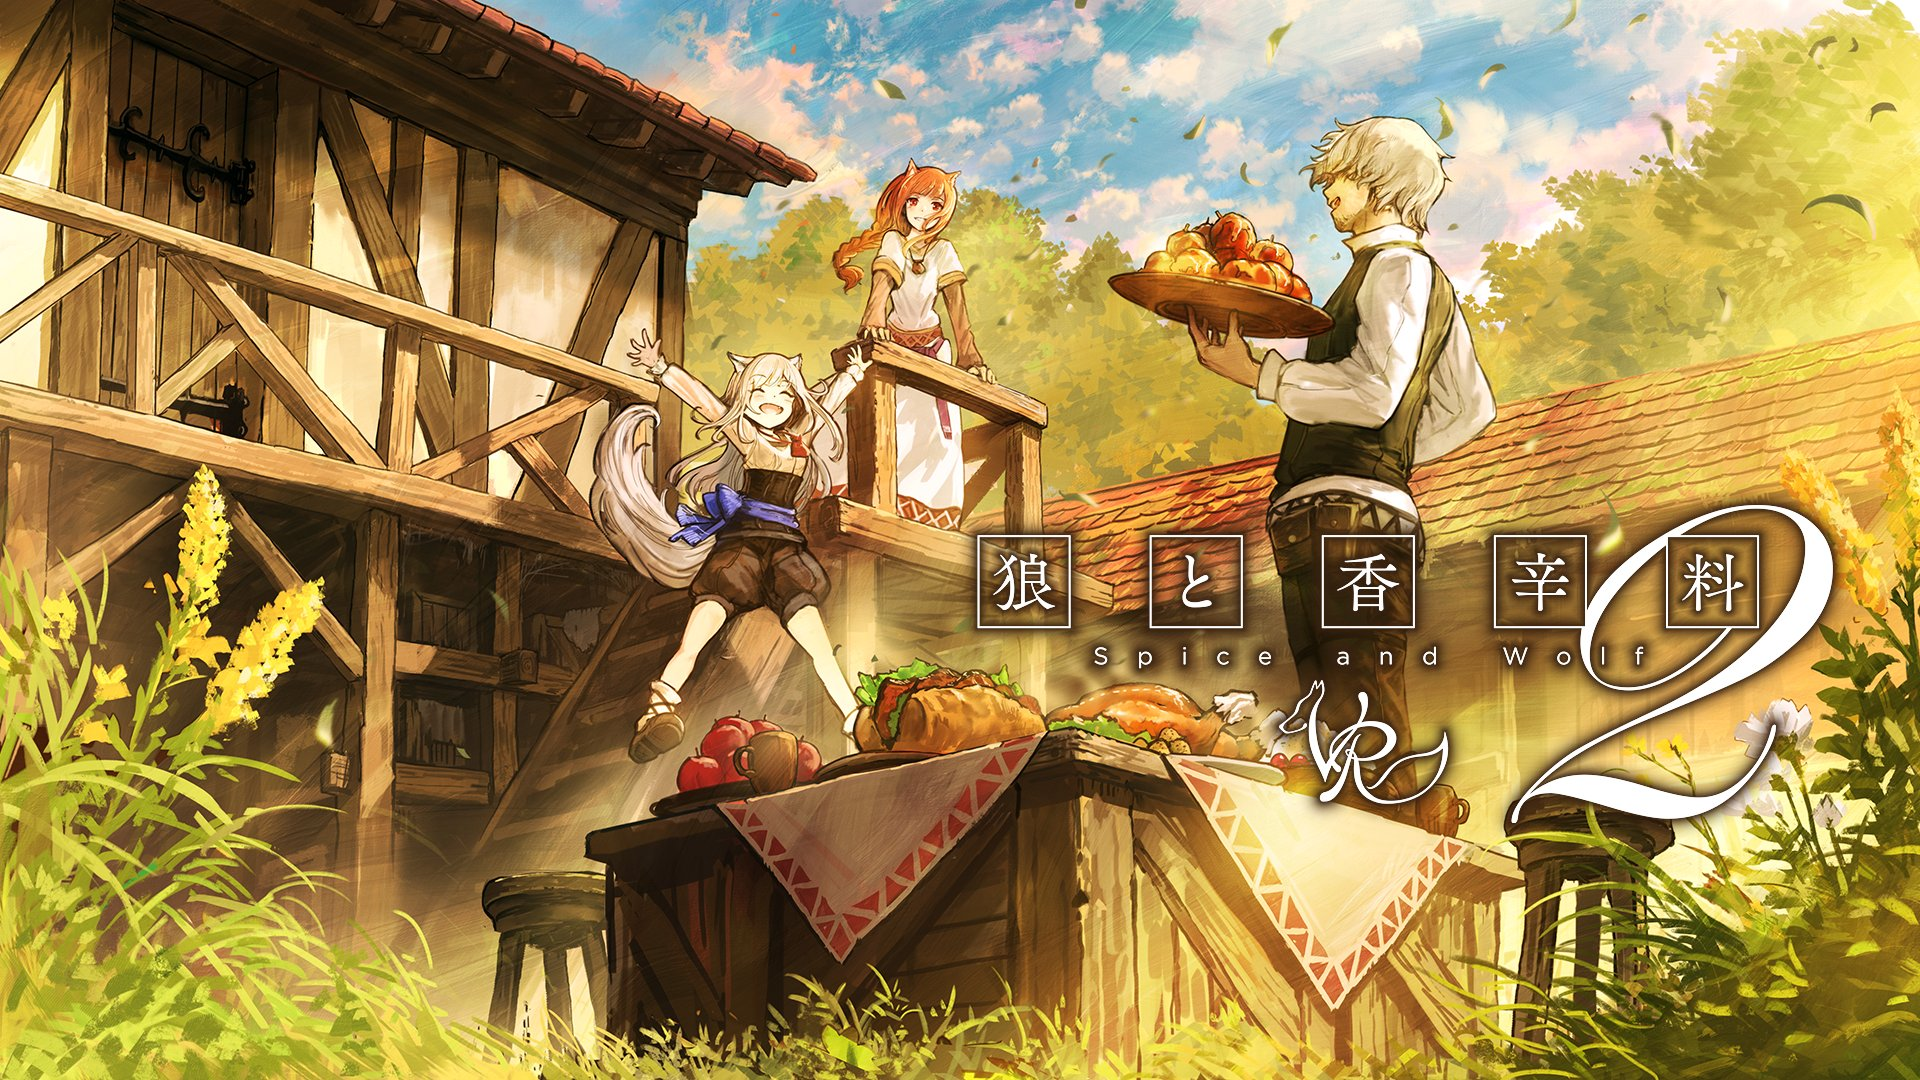
\includegraphics{EisJLXFVkAAZN1c.jpg}

\hypertarget{carga-de-libreruxedas-y-archivos}{%
\section{\texorpdfstring{\textbf{Carga de librerías y
archivos}}{Carga de librerías y archivos}}\label{carga-de-libreruxedas-y-archivos}}

\begin{center}\rule{0.5\linewidth}{0.5pt}\end{center}

Para la obtención del texto de las novelas se realizó la transcripción
de las 23 novelas ligeras a archivos de texto. Junto a estos archivos de
texto se realizó la carga de los léxicos (o lexicon en inglés) para
realizar el análisis de sentimientos. Además, para este trabajo se
necesitó herramientas de text mining, manipulación de dataframes, entre
otros, especificados a continuación:

\begin{Shaded}
\begin{Highlighting}[]
\CommentTok{#Se cargan las librerías}
\KeywordTok{library}\NormalTok{(tidyverse) }\CommentTok{#Manipulación de datos}
\KeywordTok{library}\NormalTok{(tm) }\CommentTok{#Text mining}
\KeywordTok{library}\NormalTok{(wordcloud) }\CommentTok{#Generador de nube de palabras}
\KeywordTok{library}\NormalTok{(wordcloud2) }\CommentTok{#Generador de nube de palabras}
\KeywordTok{library}\NormalTok{(tidytext) }\CommentTok{#Text mining y procesado de palabras}
\KeywordTok{library}\NormalTok{(reshape2) }\CommentTok{#Modificación a dataframes}
\KeywordTok{library}\NormalTok{(RWeka) }\CommentTok{#Data Mining y tokenizador}
\KeywordTok{library}\NormalTok{(knitr) }\CommentTok{#Generación de markdowns}
\KeywordTok{library}\NormalTok{(readtext) }\CommentTok{#Para la lectura de los txt}
\KeywordTok{library}\NormalTok{(kableExtra)}


\CommentTok{#Se cargan los archivos}
\NormalTok{FILEDIR =}\StringTok{ "data_holo/PDF/"}
\NormalTok{filenames <-}\StringTok{ }\KeywordTok{list.files}\NormalTok{(FILEDIR)}
\NormalTok{filenames <-}\StringTok{ }\KeywordTok{gsub}\NormalTok{(}\StringTok{".txt$"}\NormalTok{, }\StringTok{""}\NormalTok{, filenames)}
\NormalTok{txts <-}\StringTok{ }\KeywordTok{readtext}\NormalTok{(FILEDIR)}

\CommentTok{#Se cargan los léxicos para el análisis de sentimiento}
\NormalTok{bing <-}\StringTok{ }\KeywordTok{read_csv}\NormalTok{(}\StringTok{"data/lexi/Bing.csv"}\NormalTok{)}
\NormalTok{nrc <-}\StringTok{ }\KeywordTok{read_csv}\NormalTok{(}\StringTok{"data/lexi/NRC.csv"}\NormalTok{)}
\NormalTok{afinn <-}\StringTok{ }\KeywordTok{read_csv}\NormalTok{(}\StringTok{"data/lexi/Afinn.csv"}\NormalTok{)}
\end{Highlighting}
\end{Shaded}

\hypertarget{preprocesado-de-las-novelas}{%
\section{\texorpdfstring{\textbf{Preprocesado de las
novelas}}{Preprocesado de las novelas}}\label{preprocesado-de-las-novelas}}

\begin{center}\rule{0.5\linewidth}{0.5pt}\end{center}

Antes de realizar cualquier análisis es necesario ordenar las columnas
según su orden de publicación. Además se debe limpiar el texto para
poder utilizarlo. La limpieza consistirá en eliminar carácteres
extraños, tabulaciones, espacios, saltos de línea, números, juntar
palabras, eliminar stopwords y puntuaciones.

\end{document}
